\documentclass{report}

\usepackage[letterpaper,top=1.4cm,bottom=1.4cm,left=2.2cm,right=2.2cm,marginparwidth=1.6cm]{geometry}

\usepackage{caption}        %для картинок
\usepackage{multicol}       %для мультиколонок
\usepackage[english]{babel} %для английского языка
\usepackage[T2A]{fontenc}   %для шрифта
\usepackage[utf8]{inputenc} %для кодировки
\usepackage{titlesec}       %для стилей текста
\usepackage{graphicx}       %для графики
\graphicspath{ {./images/} }

\begin{document}        

\setcounter{page}{199}

\begin{multicols}{2}

\begin{center}
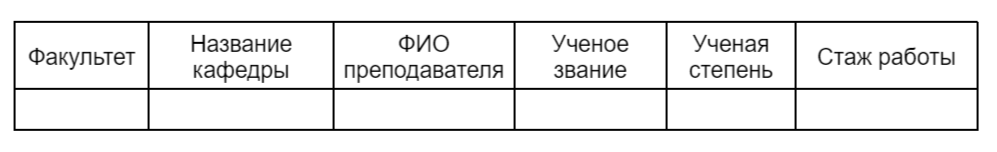
\includegraphics[width=8cm, height = 14cm]{1.png}
\parbox[c]{16.4cm}{\scriptsize{Figure 10.~}The structure of eXnet (original image from [19])}
\end{center}

\begin{itemize}
    \item [\text{}] 640x480 pixels. It should be noted, however, that
the classes for this dataset differ from the abovementioned ones (for example, instead of a neutral
emotion, there is an emotion of despisal). This was
one of the reasons why there was a need to form
a combined dataset;
    \item [\text{2)}]The ”Students and colleagues“ dataset. This
dataset was collected from data obtained by selfdetermined image collection and processing. It is
a set of images of the faces of 38 people with
the expression of basic emotions. The training part
included 20,947 images, the control part – 2,101;
    \item [\text{3)}]Internet Emotions. This dataset was formed from
images taken from the Internet and includes oneman photos of 295 people, which include training
(268 images) and control (27 images) datasets.
\end{itemize}

\par Thus, the total size of the training dataset was 25,830
images and the control one – 2,682.
\par As a result of additional training of the eXnet model
on the dataset described above, the results presented in
table I were obtained.
\par \textbf{avg valid} – the percentage of successfully recognized

\columnbreak


\begin{center}
\par Table I

\scriptsize \par {\small R}ESULTS OF TRAINING THE E{\small X}NET MODEL
\vspace{0.25cm}

\begin{tabular}{ |c|c|c| } 
 \hline 
 &\textit{\textbf{avg. valid}}&\textit{\textbf{avg. valid softmax}}\\
 \hline
 \textbf{CK+}&0.877&0.859\\
 \hline
 \textbf{Students and Colleagues}&0.765&0.742\\
 \hline
 \textbf{Internet}&0.37&0.305\\
 \hline
\end{tabular}
\end{center}

\vspace{0.1cm}

\par \noindent emotions taken as 1 in the test dataset.
\par \textbf{avg softmax} – the percentage of successfully recognized emotions, taking into account the obtained probability from the range (0..1] in the test dataset.
\par \textbf{ck+}, \textbf{student\_colleague} and \textbd{internet} denote the overall accuracy that results from the corresponding test
datasets. \textbf{average\_valid} and \textbf{average\_valid\_softmax} are
the metrics used to evaluate accuracy.
\par \noindent \textit{F. Semantic analysis}
\par The described integration mechanism allows enriching
the knowledge base with the results of recognition of
various models used by the computer vision module
(identification model and emotion recognition model).
The processing of this knowledge will be no different
from the processing of any other knowledge in the ostissystem, regardless of whether they got there from the
computer vision module, any sensors, visual or natural
language interface or in some other way. In this case,
computer vision is another receptor of the system
\par Knowledge processing in the KB, i.e., semantic analysis, is performed by the problem solver. The problem
solver is a set of agents that react to events in the
knowledge base (for example, a problem definition),
solve its problem (generating, transforming knowledge,
accessing external systems) and put the result of the work
in the same KB.
\par For example, one of the methods of knowledge processing can be the usage of logical inference [21],
which generates new knowledge based on a set of rules.
Logical rules, in the simplest case, can be represented
by “if-then” bindings, where the “if” part describes the
knowledge that must be in the knowledge base to make
it possible for us to generate the knowledge described in
the “then” part. The origin of such rules can be different:
from adding them manually by knowledge base engineers
to automatically generating them.
\par In the considered implementation of the hybrid system,
the logical rules [21] are used to generate some standard
system responses to the interlocutor’s messages. These
rules use such knowledge as the identification of the
interlocutor and their current emotion. Figure 11 shows
a fragment of such a rule in a simplified form for
clarity (in a real system, such rules have a more complex
specification).
\par The meaning of the rule is as follows: if we received
a greeting message from a user, whose emotion is recognized by the system as “sadness” and whose name the

\end{multicols}

\end{document}